% Graphic for TeX using PGF
% Title: /home/satenske/cours/AP/obj3/uml16.dia
% Creator: Dia v0.97.1
% CreationDate: Thu Sep 22 10:19:31 2011
% For: satenske
% \usepackage{tikz}
% The following commands are not supported in PSTricks at present
% We define them conditionally, so when they are implemented,
% this pgf file will use them.
\ifx\du\undefined
  \newlength{\du}
\fi
\setlength{\du}{15\unitlength}
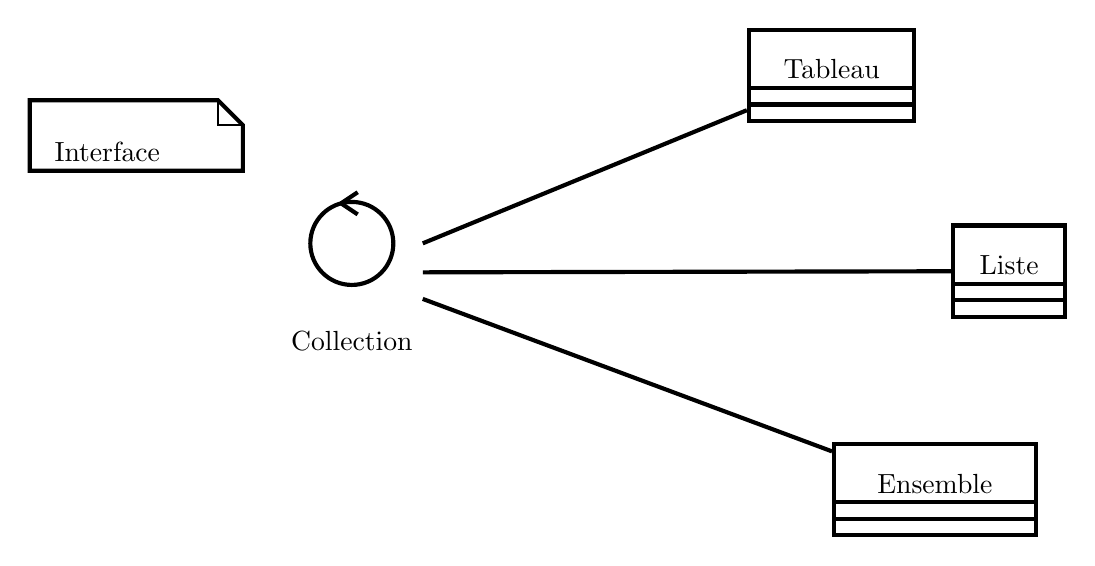
\begin{tikzpicture}
\pgftransformxscale{1.000000}
\pgftransformyscale{-1.000000}
\definecolor{dialinecolor}{rgb}{0.000000, 0.000000, 0.000000}
\pgfsetstrokecolor{dialinecolor}
\definecolor{dialinecolor}{rgb}{1.000000, 1.000000, 1.000000}
\pgfsetfillcolor{dialinecolor}
\pgfsetlinewidth{0.100000\du}
\pgfsetdash{}{0pt}
\definecolor{dialinecolor}{rgb}{1.000000, 1.000000, 1.000000}
\pgfsetfillcolor{dialinecolor}
\fill (19.675000\du,-5.885000\du)--(19.675000\du,-4.485000\du)--(23.657500\du,-4.485000\du)--(23.657500\du,-5.885000\du)--cycle;
\definecolor{dialinecolor}{rgb}{0.000000, 0.000000, 0.000000}
\pgfsetstrokecolor{dialinecolor}
\draw (19.675000\du,-5.885000\du)--(19.675000\du,-4.485000\du)--(23.657500\du,-4.485000\du)--(23.657500\du,-5.885000\du)--cycle;
% setfont left to latex
\definecolor{dialinecolor}{rgb}{0.000000, 0.000000, 0.000000}
\pgfsetstrokecolor{dialinecolor}
\node at (21.666250\du,-4.935000\du){Tableau};
\definecolor{dialinecolor}{rgb}{1.000000, 1.000000, 1.000000}
\pgfsetfillcolor{dialinecolor}
\fill (19.675000\du,-4.485000\du)--(19.675000\du,-4.085000\du)--(23.657500\du,-4.085000\du)--(23.657500\du,-4.485000\du)--cycle;
\definecolor{dialinecolor}{rgb}{0.000000, 0.000000, 0.000000}
\pgfsetstrokecolor{dialinecolor}
\draw (19.675000\du,-4.485000\du)--(19.675000\du,-4.085000\du)--(23.657500\du,-4.085000\du)--(23.657500\du,-4.485000\du)--cycle;
\definecolor{dialinecolor}{rgb}{1.000000, 1.000000, 1.000000}
\pgfsetfillcolor{dialinecolor}
\fill (19.675000\du,-4.085000\du)--(19.675000\du,-3.685000\du)--(23.657500\du,-3.685000\du)--(23.657500\du,-4.085000\du)--cycle;
\definecolor{dialinecolor}{rgb}{0.000000, 0.000000, 0.000000}
\pgfsetstrokecolor{dialinecolor}
\draw (19.675000\du,-4.085000\du)--(19.675000\du,-3.685000\du)--(23.657500\du,-3.685000\du)--(23.657500\du,-4.085000\du)--cycle;
\pgfsetlinewidth{0.100000\du}
\pgfsetdash{}{0pt}
\definecolor{dialinecolor}{rgb}{1.000000, 1.000000, 1.000000}
\pgfsetfillcolor{dialinecolor}
\fill (24.600000\du,-1.170000\du)--(24.600000\du,0.230000\du)--(27.285000\du,0.230000\du)--(27.285000\du,-1.170000\du)--cycle;
\definecolor{dialinecolor}{rgb}{0.000000, 0.000000, 0.000000}
\pgfsetstrokecolor{dialinecolor}
\draw (24.600000\du,-1.170000\du)--(24.600000\du,0.230000\du)--(27.285000\du,0.230000\du)--(27.285000\du,-1.170000\du)--cycle;
% setfont left to latex
\definecolor{dialinecolor}{rgb}{0.000000, 0.000000, 0.000000}
\pgfsetstrokecolor{dialinecolor}
\node at (25.942500\du,-0.220000\du){Liste};
\definecolor{dialinecolor}{rgb}{1.000000, 1.000000, 1.000000}
\pgfsetfillcolor{dialinecolor}
\fill (24.600000\du,0.230000\du)--(24.600000\du,0.630000\du)--(27.285000\du,0.630000\du)--(27.285000\du,0.230000\du)--cycle;
\definecolor{dialinecolor}{rgb}{0.000000, 0.000000, 0.000000}
\pgfsetstrokecolor{dialinecolor}
\draw (24.600000\du,0.230000\du)--(24.600000\du,0.630000\du)--(27.285000\du,0.630000\du)--(27.285000\du,0.230000\du)--cycle;
\definecolor{dialinecolor}{rgb}{1.000000, 1.000000, 1.000000}
\pgfsetfillcolor{dialinecolor}
\fill (24.600000\du,0.630000\du)--(24.600000\du,1.030000\du)--(27.285000\du,1.030000\du)--(27.285000\du,0.630000\du)--cycle;
\definecolor{dialinecolor}{rgb}{0.000000, 0.000000, 0.000000}
\pgfsetstrokecolor{dialinecolor}
\draw (24.600000\du,0.630000\du)--(24.600000\du,1.030000\du)--(27.285000\du,1.030000\du)--(27.285000\du,0.630000\du)--cycle;
\pgfsetlinewidth{0.100000\du}
\pgfsetdash{}{0pt}
\definecolor{dialinecolor}{rgb}{1.000000, 1.000000, 1.000000}
\pgfsetfillcolor{dialinecolor}
\fill (21.725000\du,4.095000\du)--(21.725000\du,5.495000\du)--(26.582500\du,5.495000\du)--(26.582500\du,4.095000\du)--cycle;
\definecolor{dialinecolor}{rgb}{0.000000, 0.000000, 0.000000}
\pgfsetstrokecolor{dialinecolor}
\draw (21.725000\du,4.095000\du)--(21.725000\du,5.495000\du)--(26.582500\du,5.495000\du)--(26.582500\du,4.095000\du)--cycle;
% setfont left to latex
\definecolor{dialinecolor}{rgb}{0.000000, 0.000000, 0.000000}
\pgfsetstrokecolor{dialinecolor}
\node at (24.153750\du,5.045000\du){Ensemble};
\definecolor{dialinecolor}{rgb}{1.000000, 1.000000, 1.000000}
\pgfsetfillcolor{dialinecolor}
\fill (21.725000\du,5.495000\du)--(21.725000\du,5.895000\du)--(26.582500\du,5.895000\du)--(26.582500\du,5.495000\du)--cycle;
\definecolor{dialinecolor}{rgb}{0.000000, 0.000000, 0.000000}
\pgfsetstrokecolor{dialinecolor}
\draw (21.725000\du,5.495000\du)--(21.725000\du,5.895000\du)--(26.582500\du,5.895000\du)--(26.582500\du,5.495000\du)--cycle;
\definecolor{dialinecolor}{rgb}{1.000000, 1.000000, 1.000000}
\pgfsetfillcolor{dialinecolor}
\fill (21.725000\du,5.895000\du)--(21.725000\du,6.295000\du)--(26.582500\du,6.295000\du)--(26.582500\du,5.895000\du)--cycle;
\definecolor{dialinecolor}{rgb}{0.000000, 0.000000, 0.000000}
\pgfsetstrokecolor{dialinecolor}
\draw (21.725000\du,5.895000\du)--(21.725000\du,6.295000\du)--(26.582500\du,6.295000\du)--(26.582500\du,5.895000\du)--cycle;
\definecolor{dialinecolor}{rgb}{1.000000, 1.000000, 1.000000}
\pgfsetfillcolor{dialinecolor}
\pgfpathellipse{\pgfpoint{10.108750\du}{-0.737500\du}}{\pgfpoint{1.000000\du}{0\du}}{\pgfpoint{0\du}{1.000000\du}}
\pgfusepath{fill}
\pgfsetlinewidth{0.100000\du}
\pgfsetdash{}{0pt}
\definecolor{dialinecolor}{rgb}{0.000000, 0.000000, 0.000000}
\pgfsetstrokecolor{dialinecolor}
\pgfpathellipse{\pgfpoint{10.108750\du}{-0.737500\du}}{\pgfpoint{1.000000\du}{0\du}}{\pgfpoint{0\du}{1.000000\du}}
\pgfusepath{stroke}
\definecolor{dialinecolor}{rgb}{0.000000, 0.000000, 0.000000}
\pgfsetstrokecolor{dialinecolor}
\draw (9.849931\du,-1.703426\du)--(10.249931\du,-1.436759\du);
\definecolor{dialinecolor}{rgb}{0.000000, 0.000000, 0.000000}
\pgfsetstrokecolor{dialinecolor}
\draw (9.849931\du,-1.703426\du)--(10.249931\du,-1.970092\du);
% setfont left to latex
\definecolor{dialinecolor}{rgb}{0.000000, 0.000000, 0.000000}
\pgfsetstrokecolor{dialinecolor}
\node at (10.108750\du,1.607500\du){Collection};
\pgfsetlinewidth{0.100000\du}
\pgfsetdash{}{0pt}
\pgfsetdash{}{0pt}
\pgfsetbuttcap
{
\definecolor{dialinecolor}{rgb}{0.000000, 0.000000, 0.000000}
\pgfsetfillcolor{dialinecolor}
% was here!!!
\definecolor{dialinecolor}{rgb}{0.000000, 0.000000, 0.000000}
\pgfsetstrokecolor{dialinecolor}
\draw (19.625488\du,-3.946712\du)--(11.817615\du,-0.739454\du);
}
\pgfsetlinewidth{0.100000\du}
\pgfsetdash{}{0pt}
\pgfsetdash{}{0pt}
\pgfsetbuttcap
{
\definecolor{dialinecolor}{rgb}{0.000000, 0.000000, 0.000000}
\pgfsetfillcolor{dialinecolor}
% was here!!!
\definecolor{dialinecolor}{rgb}{0.000000, 0.000000, 0.000000}
\pgfsetstrokecolor{dialinecolor}
\draw (24.550379\du,-0.067143\du)--(11.817856\du,-0.041008\du);
}
\pgfsetlinewidth{0.100000\du}
\pgfsetdash{}{0pt}
\pgfsetdash{}{0pt}
\pgfsetbuttcap
{
\definecolor{dialinecolor}{rgb}{0.000000, 0.000000, 0.000000}
\pgfsetfillcolor{dialinecolor}
% was here!!!
\definecolor{dialinecolor}{rgb}{0.000000, 0.000000, 0.000000}
\pgfsetstrokecolor{dialinecolor}
\draw (21.676330\du,4.272031\du)--(11.817227\du,0.598997\du);
}
\pgfsetlinewidth{0.100000\du}
\pgfsetdash{}{0pt}
\definecolor{dialinecolor}{rgb}{1.000000, 1.000000, 1.000000}
\pgfsetfillcolor{dialinecolor}
\fill (2.350000\du,-4.187500\du)--(6.885000\du,-4.187500\du)--(7.485000\du,-3.587500\du)--(7.485000\du,-2.487500\du)--(2.350000\du,-2.487500\du)--cycle;
\definecolor{dialinecolor}{rgb}{0.000000, 0.000000, 0.000000}
\pgfsetstrokecolor{dialinecolor}
\draw (2.350000\du,-4.187500\du)--(6.885000\du,-4.187500\du)--(7.485000\du,-3.587500\du)--(7.485000\du,-2.487500\du)--(2.350000\du,-2.487500\du)--cycle;
\pgfsetlinewidth{0.050000\du}
\definecolor{dialinecolor}{rgb}{0.000000, 0.000000, 0.000000}
\pgfsetstrokecolor{dialinecolor}
\draw (6.885000\du,-4.187500\du)--(6.885000\du,-3.587500\du)--(7.485000\du,-3.587500\du);
% setfont left to latex
\definecolor{dialinecolor}{rgb}{0.000000, 0.000000, 0.000000}
\pgfsetstrokecolor{dialinecolor}
\node[anchor=west] at (2.700000\du,-2.942500\du){Interface  };
\end{tikzpicture}
